\section{El procesador SweRV-EL2}

El procesador SweRV-EL2 ha sido creado por Western Digital y publicado por la colaboración de código abierto CHIPS Alliance\footnote{CHIPS: \textit{Common Hardware for Interfaces, Processors and Systems}} en 2020. Es la segunda generación de la familia SweRV de procesadores, siendo de estos el más ligero y menos potente. Ha sido fabricado a 16 nm en TSMC con un área total de $0.023mm^2$, y funcionando con una frecuencia objetivo de 600MHz. Su repertorio de instrucciones es el RV32IMC+Zbb+Zbs (Zbb y Zbs son instrucciones de manipulación de bits aún no ratificadas), por lo que pueden realizarse multiplicaciones y divisiones hardware.

Además del core, el procesador cuenta con otros elementos periféricos: caché de Instrucciones, \textit{Closely-Coupled Memory} (CCM) (tanto de datos, DCCM, como instrucciones, ICCM), interfaces de debug y AXI de 64 bits...

Su descripción de alto nivel está parametrizada con multitud de opciones de configuración que podemos fijar manualmente o ejecutando la herramienta \textit{swerv\_config\_gen}, por ejemplo: si queremos optimizar para FPGA, si queremos que incluya puerto AXI, el tamaño de las cachés y sus políticas de funcionamiento, la configuración del predictor de salto... La herramienta también cuenta con cuatro perfiles objetivo predefinidos:
\begin{itemize}[noitemsep]
    \item \textbf{default}: Configuración por defecto con una interfaz bus AXI4.
    \item \textbf{default\_ahb}: Configuración por defecto con una interfaz bus AHB.
    \item \textbf{typical\_pd}: Se le quita la ICCM y tiene una interfaz bus AXI4. Es la usada para la fabricación en ASIC y la única que tiene desactivadas las optimizaciones para FPGA.
    \item \textbf{high\_perf}: Configuración para alto rendimiento con interfaz bus AXI4. Para lograr un mejor rendimiento se aumentan algunos recursos, como el tamaño del \textit{Branch Target Buffer} o el \textit{Branch History Buffer}, logrando mejores predicciones de salto.
\end{itemize}

En este proyecto hemos elegido la configuración \textit{default} con optimizaciones para \mbox{FPGA}, aunque no existen motivos por los que nuestras modificaciones no funcionasen con otras configuraciones.

\subsection{Microarquitectura}
El \textit{core} del SweRV-EL2 está segmentado en 4 etapas y se emite una sola instrucción por ciclo, por lo que es \textit{escalar}. Está diseñado para conseguir un \textit{IPC} (Instrucciones por Ciclo) cercano a $1.0$, logrando $0.95\ IPC$ y $0.98\ IPC$ en las pruebas \textit{Coremark} y \textit{Dhrystone}.

La figura \ref{fig:swerv_complex} presenta un esquema de las etapas del core. En primer lugar, se ejecuta la etapa de \textit{Fetch}, en la que se obtiene la instrucción de la memoria y se guarda en unos registros. A continuación, se hace la decodificación (\textit{Decode}) de la instrucción, obteniendo la información relevante: si es una instrucción de salto, una operación aritmético-lógica, los registros fuentes y destino, el inmediato codificado, etc. Después, dependiendo del tipo de instrucción puede ejecutarse uno u otro \textit{pipe} (fase \textit{Execute}), para continuar salvando los resultados durante la fase de \textit{Commit}.

Las instrucciones de multiplicación pasarán por el \textit{multiply pipe} que hace uso del multiplicador, con una latencia de 1 ciclo. Del mismo modo, las instrucciones de división pasarán por un \textit{pipe} no segmentado que utiliza el divisor, con una latencia de 34 ciclos. El resto de instrucciones usarán el \textit{pipe} principal ---llamado \textit{I0}---, excepto las de tipo \textit{load} y \textit{store}, que también cuentan con un \textit{pipe} dedicado. 
En este proyecto hemos incluido una NoC que solo será usada por los \textit{pipes} de multiplicación y división.
% En la figura \ref{fig:swerv_complex} podemos encontrar un diagrama con las distintas fases de una instrucción.

\begin{figure}[h]
    \centering
    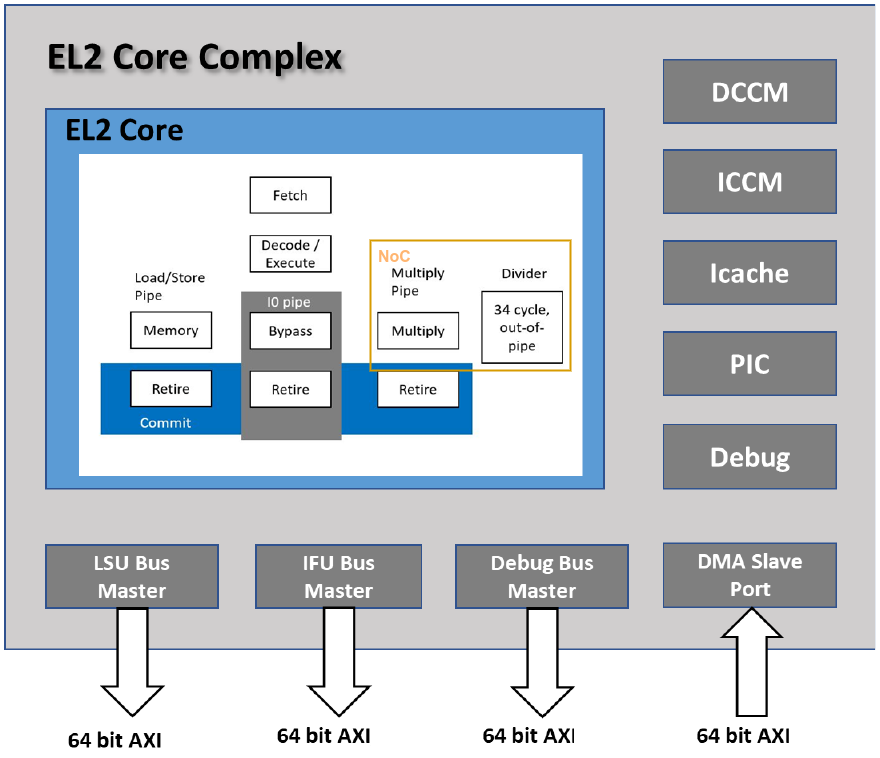
\includegraphics[width=.7\textwidth]{images/diagrams/swerv_architecture.drawio.png}
    \caption[Fases de una instrucción ejecutada en el SweRV-EL2.]{Fases de una instrucción ejecutada en el SweRV-EL2. Señalado en naranja las fases que hacen uso de la NoC. Extraído de \citetitle{SweRVRoadmap}~\cite{SweRVRoadmap}.}
    \label{fig:swerv_complex}
\end{figure}

\subsection{Diseño RTL}

En cuanto al diseño RTL, programado en SystemVerilog, el \textit{top-module} del procesador es \textit{el2\_swerv\_wrapper}, que instancia y conecta la memoria (\textit{el2\_mem}) y la interfaz DMI (\textit{dmi\_wrapper}) con el \textit{core} (\textit{el2\_swerv}).

En la figura \ref{fig:swerv_fu} se muestra el diagrama de bloques del diseño simplificado y las unidades funcionales con las que cuenta el \textit{core}, cada una con las siguientes responsabilidades:

\begin{itemize}[noitemsep]
    \item [\textbf{ifu}] \textit{Instruction Fetch Unit}. Unidad funcional encargada de la fase \textit{fetch} de una instrucción. Se conecta con la memoria y obtiene la instrucción especificada por el contador del programa.
    \item [\textbf{dec}] Se encarga de la decodificación de las instrucciones obtenidas por la \textit{ifu}, obteniendo los operandos para la \textit{exu} y manejando las señales de control de esta.
    \item [\textbf{exu}] \textit{Execution Unit}. Esta unidad funcional se encarga de ejecutar la instrucción, por lo que instancia distintos submódulos para los distintos \textit{pipes} de ejecución. Esta es la unidad funcional a la que se añadirá la NoC.
    \item [\textbf{lsu}] \textit{Load-Store Unit}. Se encarga de ejecutar las instrucciones de \textit{load} y \textit{store}, accediendo a la memoria.
\end{itemize}

En este proyecto añadiremos una NoC para conectar los submódulos de la EXU, que se explican más en profundidad en la sección \hyperref[subsec:exu_mods]{\ref{subsec:exu_mods}~\nameref{subsec:exu_mods}}.

\begin{figure}[h]
    \centering
    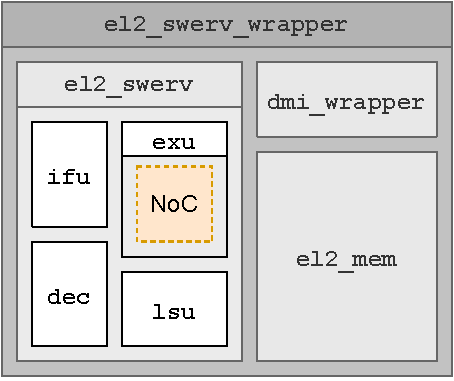
\includegraphics{images/schematics/swerv_blocks.drawio.pdf}
    % \missingfigure{Aquí pondré una figura con las distintas unidades funcionales del SweRV, y la NoC dibujada dentro de la ALU (sin mucho detalle)}
    \caption{Diagrama de bloques simplificado del diseño RTL del SweRV-EL2, mostrando las unidades funcionales del \textit{core}. En naranja se muestra la ubicación de la NoC añadida.}
    \label{fig:swerv_fu}
\end{figure}
